% Shared standalone design for the editable figure reconstructions.
\documentclass[tikz,border=5pt,10pt]{standalone}
\usepackage[T1]{fontenc}
\usepackage[utf8]{inputenc}
\usepackage{newpxtext,newpxmath}
\usepackage[scaled=.94]{sourcesanspro}
\usepackage{pgfplots}
\pgfplotsset{compat=1.18}
\usetikzlibrary{arrows.meta,calc,positioning,decorations.pathreplacing,
  decorations.markings,patterns,matrix,shapes.geometric,fit,backgrounds,
  intersections,angles,quotes}
\definecolor{ink}{HTML}{203746}
\definecolor{accent}{HTML}{146C78}
\definecolor{muted}{HTML}{667780}
\definecolor{signalred}{HTML}{B94B44}
\color{ink}
\tikzset{>=Latex,line width=.8pt,
  every node/.style={font=\small},
  axis/.style={->,draw=muted,line width=.5pt},
  guide/.style={draw=muted,dashed,line width=.45pt},
  curve/.style={draw=accent,line width=1pt},
  marker/.style={circle,fill=accent,inner sep=1.5pt},
  labelbox/.style={fill=white,inner sep=2pt}}

\begin{document}
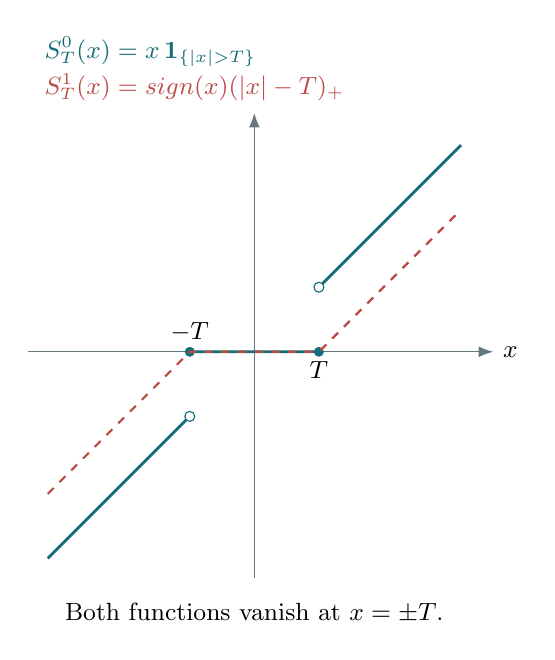
\begin{tikzpicture}[x=.82cm,y=.82cm]
\draw[axis] (-3.5,0)--(3.7,0) node[right] {$x$};\draw[axis] (0,-3.5)--(0,3.7) node[above] {$$};
\draw[curve] (-3.2,-3.2)--(-1,-1) (1,1)--(3.2,3.2) (-1,0)--(1,0);
\foreach \u/\v in {-1/-1,1/1}{\draw[accent,fill=white] (\u,\v) circle(1.8pt);}
\foreach \u in {-1,1}{\fill[accent] (\u,0) circle(1.8pt);}
\draw[signalred,dashed,thick] (-3.2,-2.2)--(-1,0)--(1,0)--(3.2,2.2);
\node[above] at (-1,0) {$-T$};\node[below] at (1,0) {$T$};
\node[accent,anchor=west] at (-3.4,4.65) {$S_T^0(x)=x\,\mathbf1_{\{|x|>T\}}$};
\node[signalred,anchor=west] at (-3.4,4.1) {$S_T^1(x)=\operatorname{sign}(x)(|x|-T)_+$};
\node at (0,-4.05) {Both functions vanish at $x=\pm T$.};
\end{tikzpicture}
\end{document}
